\documentclass{article}
\usepackage{amsmath}
\usepackage{amssymb}
\usepackage{booktabs}
\usepackage{xintexpr}
\usepackage{subcaption}
\usepackage{float}
\usepackage{enumitem}
\usepackage{tikz}
\usetikzlibrary{arrows,automata,positioning}

\newcommand{\T}{1}
\newcommand{\F}{0}
\newcommand{\TF}[1]{\if1#1\T\else\F\fi}
\newcommand{\xintTF}[1]{\xintifboolexpr{#1}{\T}{\F}}

\newcommand{\logicrule}[2]{
\begin{array}{l}
#1 \\
\midrule
\therefore #2 \\
\end{array}
}

\newcommand{\inv}[1]{#1^{-1}}

\renewcommand{\d}[1]{\,\textnormal{d}#1}
\newcommand{\dd}[2]{\frac{\d{#1}}{\d{#2}}}
\newcommand{\ddd}[2]{\dfrac{\d{#1}}{\d{#2}}}

\DeclareMathOperator{\var}{Var}
\DeclareMathOperator{\E}{\mathcal{E}}

\newcommand{\multistep}[1]{\begin{array}{rl} #1 \end{array}}
\newcommand{\subeq}{\subseteq}
\newcommand{\sub}{\subset}

\newcommand{\conj}[1]{\overline{#1}}

\setlength\parindent{0pt}
\setlength\parskip{1em}

\begin{document}

\section*{Informal Description of Push Down Automata}

$M_2$ should recognize $\{a^ib^jc^k|i,j,k>0\wedge{}i=j\vee{}i=k\}$.

PDA read and push $a$'s on stack.

Then, we can match $a$'s with $b$'s or $c$'s.

Nondeterminism helps since we cannot know inadvance whether $a$'s
match $b$'s or $c$'s.

Machine can guess (2 branches - one for each guess).

If either branch matches that branch accepts and entire machine
accepts.

\subsection*{Transition Diagram}

\begin{figure}[H]
  \centering
  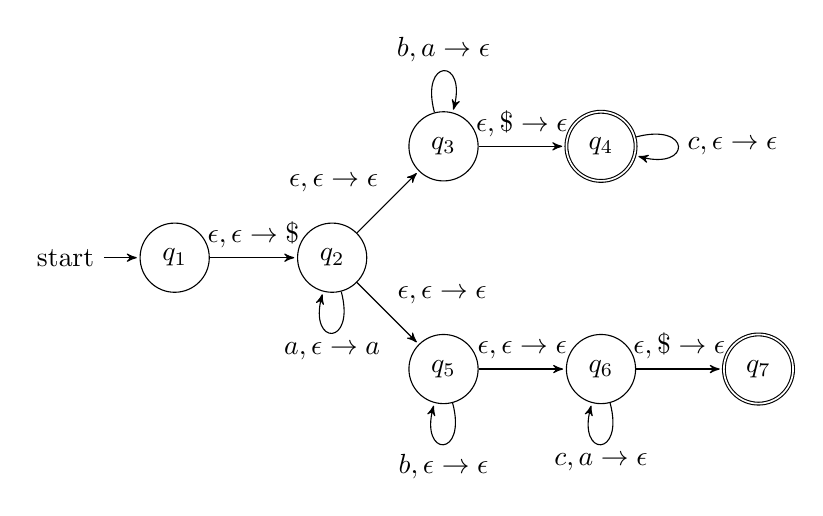
\begin{tikzpicture}[>=stealth',shorten >=1pt,auto,node distance=2cm]
    \node[initial,state] (q1) {$q_1$};
    \node[state] (q2) [right of=q1] {$q_2$};
    \node[state] (q3) [above right of=q2] {$q_3$};
    \node[state,accepting] (q4) [right of=q3] {$q_4$};
    \node[state] (q5) [below right of=q2] {$q_5$};
    \node[state] (q6) [right of=q5] {$q_6$};
    \node[state,accepting] (q7) [right of=q6] {$q_7$};

    \path[->]
    (q1) edge node {$\epsilon,\epsilon\rightarrow\$$} (q2)

    (q2) edge [loop below] node {$a,\epsilon\rightarrow{}a$} (q2)
    (q2) edge node {$\epsilon,\epsilon\rightarrow\epsilon$} (q3)
    (q2) edge node {$\epsilon,\epsilon\rightarrow\epsilon$} (q5)

    (q3) edge [loop above] node {$b,a\rightarrow\epsilon$} (q3)
    (q3) edge node {$\epsilon,\$\rightarrow\epsilon$} (q4)

    (q4) edge [loop right] node {$c,\epsilon\rightarrow\epsilon$} (q4)

    (q5) edge [loop below] node {$b,\epsilon\rightarrow\epsilon$} (q5)
    (q5) edge node {$\epsilon,\epsilon\rightarrow\epsilon$} (q6)

    (q6) edge [loop below] node {$c,a\rightarrow\epsilon$} (q6)
    (q6) edge node {$\epsilon,\$\rightarrow\epsilon$} (q7)
    ;
  \end{tikzpicture}
  \caption{$M_2$}
\end{figure}

\end{document}
